%&program=pdflatex
%%%%%%%%%%%%%%%%%%%%%%%%%%%%%%%%%%%%%%%%%%%%%%%%%%%%%%%%%%%%%%%%%%%%%%%%%%%%%%%%
% VIGIL AND LAW OF A ROVER SCOUT
%
% KNOWN TYPOGRAPHY ISSUES
%  * This should probably be XeTeX'd and should probabaly use something like
%    Hoeflr Text, or anything that isn't ``Modern''.  That may help it not 
%    like a piece of techinical documentation...
%%%%%%%%%%%%%%%%%%%%%%%%%%%%%%%%%%%%%%%%%%%%%%%%%%%%%%%%%%%%%%%%%%%%%%%%%%%%%%%%

\documentclass[11pt]{article}
\usepackage{geometry}
\geometry{a4paper}
%\geometry{landscape}
%\geometry{twocolumn}


% For more Maths symbols
\usepackage{amsmath}
\usepackage{amssymb}

% For importing sweet eps
\usepackage{epstopdf}

\usepackage{graphicx}

% For sweet pseudo code
\usepackage{algorithmic}
\usepackage{algorithm}

% Sweet hyper references.
\usepackage{hyperref}

%%%%%%%%%%%%%%%%%%%%%%%%%%%%%%%%%%%%%%%%%%%%%%%%%%%%%%%%%%%%%%%%%%%%%%%%%%%%%%%%
%%%%%%%%%%%%%%%%%% STYLE OPTIONS %%%%%%%%%%%%%%%%%%%%%%%%%%%%%%%%%%%%%%%%%%%%%%%
%%%%%%%%%%%%%%%%%%%%%%%%%%%%%%%%%%%%%%%%%%%%%%%%%%%%%%%%%%%%%%%%%%%%%%%%%%%%%%%%

% Most of this crap was removed...
% probably should be readded... so it doesn't look like a Uni maths assignment.

\linespread{1.05} 

%%%%%%%%%%%%%%%%%%%%%%%%%%%%%%%%%%%%%%%%%%%%%%%%%%%%%%%%%%%%%%%%%%%%%%%%%%%%%%%%
%%%%%%%%%%%%%%%%%% END STYLE OPTIONS %%%%%%%%%%%%%%%%%%%%%%%%%%%%%%%%%%%%%%%%%%%
%%%%%%%%%%%%%%%%%%%%%%%%%%%%%%%%%%%%%%%%%%%%%%%%%%%%%%%%%%%%%%%%%%%%%%%%%%%%%%%%

%\myname command
\newcommand{\myname} {Huw Rowlands}

%\thismonth shows this month.
\newcommand{\thismonth}{
	\ifcase\month\or
  		January\or February\or March\or April\or May\or June\or
  		July\or August\or September\or October\or November\or December
	\fi
	\space\number\year}

%Make date format of \today command Australian.
\renewcommand{\today}{\number\day\space
	\ifcase\month\or
  		January\or February\or March\or April\or May\or June\or
  		July\or August\or September\or October\or November\or December
	\fi\space
	\number\year}

	
%oldtoday is just like \today, but with old style numbers and small cap months
\newcommand{\oldtoday}{\oldstylenums{\number\day}\space
	\textsc{
	\ifcase\month\or
  		January\or February\or March\or April\or May\or June\or
  		July\or August\or September\or October\or November\or December
	\fi\space}
	\oldstylenums{\number\year}}



%Set up meta data for document.
\hypersetup{
    bookmarks=true,			% show bookmarks bar?
    unicode=true,			% non-Latin characters in Acrobat's bookmarks
    pdftoolbar=true,			% show Acrobat's toolbar?
    pdfmenubar=true,			% show Acrobat's menu?
    pdffitwindow=false,		% window fit to page when opened
    pdfstartview={FitH},		% fits the width of the page to the window
    pdftitle={The Vigil and Law of a Rover Scout},		% title
    pdfauthor={Lord Baden-Powell},		% author
    pdfsubject={The Vigil and Law of a Rover Scout},			% subject of the document
    pdfcreator={\myname, Crew Leader 2011, Murrumbidgee Rover Crew},	% creator of the document
    pdfproducer={Murrumbidgee Rover Crew, ACT Branch, Scouts Australia},	% producer of the document
    pdfkeywords={},			% list of keywords
    pdfnewwindow=true,		% links in new window
    colorlinks=false,		% false: boxed links; true: colored links
    linkcolor=red,			% color of internal links
    citecolor=green,			% color of links to bibliography
    filecolor=magenta,		% color of file links
    urlcolor=cyan,			% color of external links
    linkbordercolor={1 1 1},	% color of internal links' borders
    citebordercolor={1 1 1},	% color of links to biliography's borders
    filebordercolor={1 1 1},	% color of file links' borders
    urlbordercolor={0 1 1},	% color of external links' borders
}


%%% TITLE 
\title{The Vigil and Law of a Rover Scout}%Don't forget to change the title in hypersetup section!
\author{Robert Baden-Powell, 1st Baron Baden-Powell \\ \small{\textsc{om, gcmg, gcvo, kcb}}}
\date{ 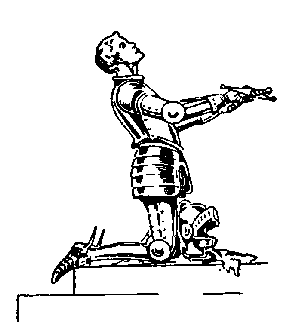
\includegraphics[width=0.32\textwidth]{knight} } % edit month above.

%%% BEGIN DOCUMENT
\begin{document}

%%% MAKE TITLE
\maketitle

\pagebreak

\tableofcontents


\break
%%% THE SCOUT LAW AND PROMISE
\section{The Scout Law and Promise}

%The Law
\subsection{The Law}
The term Rover Scouts stands for a true man and a good citizen. The Law of Rovers is the same as for Scouts, in wording and in principle, but has to be viewed from a new standpoint---that is, from that of a Man. In both cases the principle underlying the Scout Law knocks out Self and shoves in Good-will and Helpfulness to others. Don't take this as an instruction in Piety, but as a direction to Manliness.

What kind of Service am I best fitted to?
\begin{enumerate}
  \item At home?
  \item At work?
  \item In my spare time?
\end{enumerate}

As the success of our Service will depend to a great extent on our personal character, we must discipline ourselves in order that we may be a good influence to others.
\begin{enumerate}
  \item Am I determined to try and give up the bad habits I've acquired in the past?
  \item What are the weak points in my character?
  \item Am I absolutely honourable, truthful and trustworthy?
  \item Am I loyal to God, and the Queen, my Country, my family, my employers, those under me, the Scout Movement, my friends and myself?
  \item Am I good tempered, cheery and kindly to others?
  \item Am I sober clean-living, and clean-speaking?
  \item Have I pluck and patience to stick it out when things go against me?
  \item Have I a mind of my own, or do I allow myself to be carried away by the persuasion of others?
  \item Am I strong-minded enough to keep off temptation---to gamble, to drink, to harm a girl or woman?
  \item If I am weak in some of these things, do I resolve here and now, with God's help, to do my best to correct them and chock them up?
\end{enumerate}

May God give me strength to go forward henceforth a real man, a true citizen, and a credit to my country.

%Thoughts to consider during the Vigil
\subsection{Thoughts to consider during the Vigil}
As one grows older, time passes more and more quickly. Comparatively speaking, life only lasts for a short time and it is soon away. Indeed, it may end tomorrow---even this night.

\begin{enumerate}
  \item Am I making the best use of the life that God has given me?
  \item Am I frittering it away, doing nothing that counts; that is, wasting it?
  \item Am I working at things that are not doing good to anybody?
  \item Am I seeking to much my own enjoyment or money-making or promotion without trying to help other people?
  \item Whom have I injured or hurt in my life? Can I do anything to make amends?
  \item Whom have I helped in my life? Is there anyone else I can help?
\end{enumerate}

We get no pay or reward for doing service, but that makes us free men in doing it. We are not working for an employer but for God and our own conscience. This means we are Men.

The Rover Scout Section if the Scout Movement is described as a ``Brotherhood of Service'', so if we join it we will get the opportunity if training for and of doing service in many ways that would not have been open to us otherwise.

Service is not for spare time only. We must constantly on the lookout for opportunities of serving at all times.

\begin{enumerate}
  \item Am I only joining the Rover Crew for the fun I can get out of it?
  \item Am I determined to put real self-sacrificing Service into it?
  \item What do I mean by Service?
  \item Do I really think for others, rather than for myself, in my plans or undertakings?
\end{enumerate}
 
\subsubsection{A Scouts Honour is to be trusted}
As a Rover Scout, no temptation, however great or however secret, will persuade you to do a dishonest or a shady action, however small. You won't go back on a promise once made 

\begin{quote}
  ``A Rover's word is as good as his bond.''
\end{quote}
\begin{quote}
  ``The Truth, and nothing but the Truth for the Rover.''
\end{quote}

\subsubsection{A Scout is loyal to his Queen, his County, his Scouters, his Parents, and to those under him}
As a good citizen you are one of a team ``playing the game'' honestly for the good of the whole. You can be relied upon by the Queen, as head of the Empire, by the Scout Movement, by your friends and fellow workers, by your employers, to do your best for them---even though you may not always quite come up to what you would like of them. Moreover, you are loyal also to yourself; you won't lower your self-respect by playing the game meanly; nor will you let another man down---nor woman, either.

\subsubsection{A Scout's duty is to be useful and to help others}
As a Rover your highest aim is \textsc{service}. You may be relied upon at all times to be ready to sacrifice time, trouble or, if need be, like itself for others.

\begin{quote}
  ``Sacrifice is the salt of Service''
\end{quote}

\subsubsection{A Scout is thrifty}
As a Rover you will look ahead and will not fritter away time or money on present pleasures, but rather make use of present \textsc{opportunties} with a view to ultimate success. You will do this with the idea of not being a burden, but a help to others.

\subsubsection{A Scout if a friend to all, and a brother to every other Scout, no matter to what country, class or creed the other may belong.}
As a Rover, you recognise other fellows as being, with yourself, sons of the same Father, and you disregard whatever may be their difference of opinion or caste, creed or country. You suppress your prejudices and find out what their good points; any fool can criticise their bad ones. If you exercise this love for men of other countries and help to bring about international peace and good-will, that is God's Kingdom on earth.

\begin{quote}
  ``All the world's a Brotherhood''
\end{quote}

\subsubsection{A Scout is courteous}
Like a knight of old, as a Rover you are, of course, polite and considerate to women, old people and children. But more than this, you are polite also to those in opposition to you.

\begin{quote}
  ``Whoso is in the right need not lose his temper; whoso is in the wrong cannot afford to''
\end{quote}
  
\subsubsection{A Scout is a Friend to animals}
You will recognise your comradeship with God's other creatures placed, like yourself, in this world for a time to enjoy their existence. To ill-treat an animal is therefore a disservice to the creator

\subsubsection{A Scout obeys orders of his Parents, Patrol Leader or Scoutmaster without question}
As a Rover you discipline yourself and put yourself readily and willingly at the service of constituted authority for the main good. The best disciplined community is the happiest community, but the discipline must come from within, and not merely be imposed from without. Hence the greater values of the example you give to others in this direction.
 
Scouting in all its branches is voluntary and this cannot be made to clear to would-be Rover Scouts.

In his self examination the young man reviews the past, thinks of the future possibilities dimly seen, and dedicates himself in silence to the service of God, and his fellow men. Without this the Rover Scout Investiture cannot be what it is meant to be---an outward sign of an inward change of attitude to life in the world.

There need be no ceremony about this as he can keep his Vigil in the quiet of his own room, but it is the Rover Scout Leaders responsibility to see that no young man joins the Rover Scout Section of the Scout Brotherhood without being fully determined to shape his life in accordance with the Rover Scout Ideals.

When the Crews think that the Vigil should take a more definite form, it may be kept in a Church or Chapel, in the open air, in the Rover Scout Den, or indeed in any place where quiet is assured.

In such cases the Rover Scout Leader might accompany the young man to the place of the Vigil, and his two sponsors might also be present. The Rover Scout Leader and the sponsors should then retire, if desired, arrangements being made to see there is no interruption, and s leave the young man to consider the questions himself.

Whatever plan is adopted, simplicity and sincerity should be the key notes.


%NOTES ON THE VIGIL OF A ROVER SCOUT
\section{Notes on the Vigil of a Rover Scout}
This pamphlet, drawn up by the Founder, Lord Baden Powell, is a suggestion for the Vigil or self examination which precedes the investiture. It is intended to apply both those who have not previously been Scout and to those who come up from the Senior Scout Troop, for in each case they should be fully aware of the step they are taking.

The degree of ceremony used in the Vigil and the Investiture will vary, and must depend upon the wishes of the Crew and of the individual to be invested.

\subsection{The Vigil}
The central idea is that the young man before becoming a Rover Scout shall, with the aid of questions drawn up by Lord Baden Powell, quietly think about what he is doing with his life, and whether he is prepared to be invested as a Rover Scout, making his Scout Promise from the man's point of view.

The Vigil should come at the end of a period of Probation and before the Investiture.

It should be made clear to the young man that he should not be invested and the Promise made until he is quite sure that he can honestly do so. The Rover Scout Leader should point out that a sound fellow thinks carefully before he takes to a serious Promise until he has resolved to do his best to keep it.


\subsubsection{A Scout is Clean in Thought, Word and Deed}
As a Rover, you are expected to be not only clean-minded, but clean willed; able to control any sex tendencies and intemperances; to give an example to others of being pure and above board in all that you think, say and do.

There is to the Scout code an eleventh Law, an unwritten one, namely, ``a Scout is not a fool''. But this I should hope would be unnecessary in a code for Rovers. Still, as a Rover you have to remember that in crossing the threshold from boyhood into being a man you are no longer learning to carry out the Scout Law, but are actually using it for guidance of your conduct in life. More than this, you are now in the responsible position of giving an example to other, which may lead them to good or to evil, according to whether or not you model your conduct on the Law, and how far you carry that promise which you have mad, on your honour, as a Rover Scout, to give out good-will and to help all.


%THE PROMISE
\section{The Promise}


\begin{tabular}{ l p{8.5cm} }
  On my honour                     & Your honour must be a very sacred thing to you, a thing that will rule your conduct as a man. It means that you can be trusted implicitly to do what you know is right or what you agree to undertake.\\[3pt]
  I promise                        & This particular promise is a solemn undertaking, not to be made lightly even by a boy, much less so by a man. Therefore, think it over carefully before embarking on it.\\[3pt]
  To do my best                    & This means though circumstances may hinder you from doing it as completely as you with, you will, at any rate, try your upmost.\\[3pt]
  To do my duty to God             & To put if briefly, it would seem to be to try in the first place to realise the nature of God, and secondly, to develop and use, for good purposes only, the body which He has leant you, to develop the talents of mind and intelligence with which He has endowed you and, especially, to cultivate by continual practice the spirit of love and good-will to others the part of Him with is within you; that is, your soul.\\[3pt]
  And to [The Queen of] Australia  & That is, to your country, under the leadership constituted by the will of the majority.\\[3pt]
  To help other people             & This putting into constant and active practice the divine law of loving your neighbour as yourself.\\[3pt]
  And to live by the Scout Law.    & To obey the Scout Law does not mean to sit down passively in a state off goodness. But to improve your own character and actively to practise Love (which underlies the Law) in all your daily doings.\\
\end{tabular}

\subsection{A Modern Australian Promise}
\begin{verse}
  On my honour\\
  I promise\\
  To do my best\\
  To do my duty\\
  To my God\\
  And to [The Queen of] Australia\\
  To help other people\\
  And to live by the Scout Law.
\end{verse}


\end{document} 
